\section{Access control} The BI-DBS portal uses role-based access control \cite{role-auth}. In the third chapter I have designed the roles system and described their permissions. With the use of that system I have implemented the regulation of displaying the components and controlling access by roles and also verification of users' authorization for accessing components and making requests.

\subsection{Role-based access control} Vue Router is first of all responsible for displaying the components by the given path. However, it has multiple other features which I have used for my implementation.\\
Firstly it allows dynamically setting of different parameters in meta object, you can see the example of a component configuration and meta object in listing 4.4.\\

\noindent \textbf{Meta parameters for the component:}

\begin{itemize}
    \item \emph{requireAuth:} This flag simply tells if authorization is required for accessing the component.
    \item \emph{allowAccess:} This flag specifies the role that has permission to that component.
    \item \emph{sidebar:} Sidebar parameter tells the name of the configuration for navigation sidebar items.
    \item \emph{showSideBar:} This attribute is defining whether the navigation sidebar should be displayed.
    \item \emph{showTopBar:} This flag is used for the configuration of the top navigation bar and it makes clear if that bar should be displayed for that component.
\end{itemize}

\begin{lstlisting}[language=Octave, caption=The example of component configuration in Router]
{
    path: '/administration',
    component: ImportSemester,
    meta: {
    requireAuth: true,
        allowAccess: Role.GUARANTOR,
        sidebar: 'administration',
        showSideBar: true,
        showTopBar: true
    }
}
\end{lstlisting}

\noindent First two meta parameters are used for the access control, which is implemented as Router configuration. The Router allows to set a set of functionalities before each routing which I have used for the verification of a user's access to the component. This validation is presented in listing 4.5.


\begin{lstlisting}[language=Octave, caption=Validation of access by role]
export function configureGuard() {
    Router.beforeEach((to, from, next) => {
        if (to.meta.requireAuth === false) {
            next()
        } else if(verifyAccess(to, from)){
            next()
        }
    })
}

function verifyAccess(to: RouteLocationNormalized, from: RouteLocationNormalized) {
    const userStore = useUserStore()
    userStore.setPreviousPage(from.path)
        
    if (!userStore.isLoggedIn) {
        login()
    } else {
        if (userStore.user.exp_time < new Date()) {
            refreshToken()
        } else {
            return verifyRole(to)
        }
    }
    return false
}

function verifyRole(to: RouteLocationNormalized) {
    if (to.meta.allowAccess == undefined || hasRole(to.meta.allowAccess as Role)) {
        return true
    } else {
        Router.push('/error403')
        return false
    }
}
\end{lstlisting}

\noindent Firstly this configuration checks the users' authorization status if the authorization is required for the component. Secondly, it verifies that a user does have permission to access this component. In a case user is trying to access some component directly without having access they will be redirected to the error page with an option to get to the previous page, the error component is shown in figure 4.5.

\begin{figure}[hp]
\centering
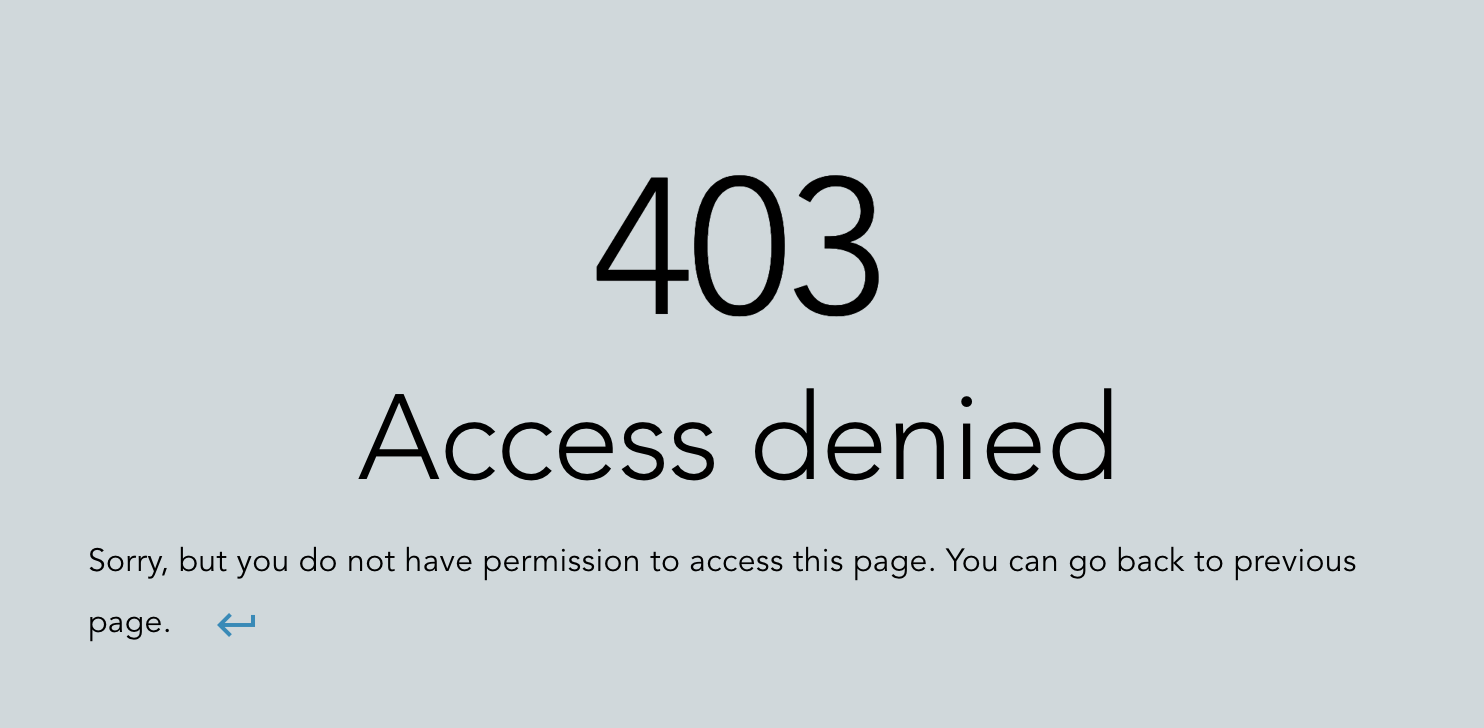
\includegraphics[scale=0.5]{../png/access_denied.png}
\caption{Access denied component}
\end{figure}



\paragraph*{Display control of components.} Another example of role-based access control benefits and usage is using it for the display control of UI components. A developer can easily control displaying of any component by setting the required role for it and using the \texttt{hasRole()} function shown in listing 4.6. The code listing 4.7. shows exactly the case like that. In the top navigation bar configuration I have set the required role for displaying the administration component and used a filter for displaying only the components user has access to.

\begin{lstlisting}[language=Octave, caption=Role validation]
export function hasRole(role: RoleTOBE) : boolean {
    switch (role) {
        case RoleTOBE.GUARANTOR:
            return isGuarantor()
        case RoleTOBE.TEACHER:
            return isStudent()
        case RoleTOBE.STUDENT:
            return isTeacher()
        default:
            return false
    }
}
\end{lstlisting}


\begin{lstlisting}[language=Octave, caption=Filtering displayed components by role]
function useTopBarConfig() {
    return computed(() => {
        const { t } = useI18n()
        return {
            tabs: [
                { name: t('base.home'), path: '/' },
                { name: t('admin.administration'), path: '/administration' , allowAccess: Role.GUARANTOR },
            ].filter(item => item.allowAccess == undefined || hasRole(item.allowAccess))
        }
    })
}
\end{lstlisting}



\noindent The implementation of regulating accesses and displaying components is clear, flexible and easy to use. It is possible due to the role-based access control, which allows simplified permissions management. Moreover, such system decreases the risk of data leaking and provides good visibility over the application.


\

\subsection{Authentication control for requests} Another important validation is verification of access for making requests to avoid the pointless calling of backend services when the user is not authorized or the access token has expired. Especially in the case when the access token has expired we need to detect it and execute the refresh process.\\
In 4.3.2.2 I have provided a code listing 4.3 of the configuration of the Axios interceptors for the request. That configuration contains a \texttt{verifyAccess()} function which makes sure the user is authorized before making the request. That function is illustrated in listing 4.8.\\


\begin{lstlisting}[language=Octave, caption=Access verification for making requests]
function verifyAccess() : Promise<string>{
    return new Promise((resolve, reject) => {
        const userStore = useUserStore()
        
        if(!userStore.isLoggedIn){
            reject('Unauthorized')
        } else if (userStore.user.exp_time < new Date()) {
            Auth.refreshToken({
                access_token: userStore.token
            }).then((response) => {
                processResponseToken(response.data.access_token)
                resolve(userStore.token)
            }).catch(() => {
                reject('Unauthorized')
            })
        } else {
            resolve(userStore.token)
        }
    })
}
\end{lstlisting}
